\documentclass{article}
\usepackage{listings}% -- Basic formatting
\usepackage[brazilian]{babel}
\usepackage[utf8]{inputenc}
\usepackage[T1]{fontenc}
\usepackage{times}
\setlength{\parindent}{8pt}
\usepackage{indentfirst}% -- Defining colors:
\usepackage[dvipsnames]{xcolor}
\definecolor{codegreen}{rgb}{0,0.6,0}
\definecolor{codegray}{rgb}{0.5,0.5,0.5}
\definecolor{codepurple}{rgb}{0.58,0,0.82}
\definecolor{backcolour}{rgb}{0.95,0.95,0.92}% Definig a custom style:
\lstdefinestyle{mystyle}{
backgroundcolor=\color{backcolour},   
commentstyle=\color{codepurple},
keywordstyle=\color{NavyBlue},
numberstyle=\tiny\color{codegray},
stringstyle=\color{codepurple},
basicstyle=\ttfamily\footnotesize\bfseries,
breakatwhitespace=false,         
breaklines=true,                 
captionpos=t,                    
keepspaces=true,                 
numbers=left,                    
numbersep=5pt,                  
showspaces=false,                
showstringspaces=false,
showtabs=false,                  
tabsize=2
}% -- Setting up the custom style:
\lstset{style=mystyle}
\usepackage{amsmath}
\usepackage{array}
\usepackage{graphicx} % Required for inserting images
\usepackage[colorlinks=true, linkcolor=blue]{hyperref}

\title{TDE 2}
\author{Gabriela Dellamora Paim}
\date{2024/06/05}

\begin{document}
\maketitle
\textbf{Observação:}
Todo o desenvolvimento está disponível no meu \href{https://github.com/MarnieGrenat/Inferencia-Comparada-2/blob/main/questao-1.R}{repositório do GitHub}. Ainda assim, disponibilizei o código nas últimas páginas.
\newpage
\section*{Questão 1 - Considere a distribuição triangular apresentada na Seção de Distribuição Triangular tal que sua função
distribuição acumulada inversa no intervalo [a, b] com moda m é dada por
\[
F^{-1}(u | a,b,m) = \begin{cases} 
a + \sqrt{u(m-a)(b-a)}, & 0 \leq u \leq \frac{m-a}{b-a} \\
b - \sqrt{(1 - u)(b - m)(b - a)}, & \frac{m-a}{b-a} < u \leq 1
\end{cases}
\]
}

\subsection*{a) Simule a densidade de uma Triangular(0, 1, 2) a partir do Método da Transformação Inversa.}

\textbf{Resposta:}

Segue uma imagem comparativa entre RTriang (função da biblioteca EnvStats) e ITriang (construída para essa questão).

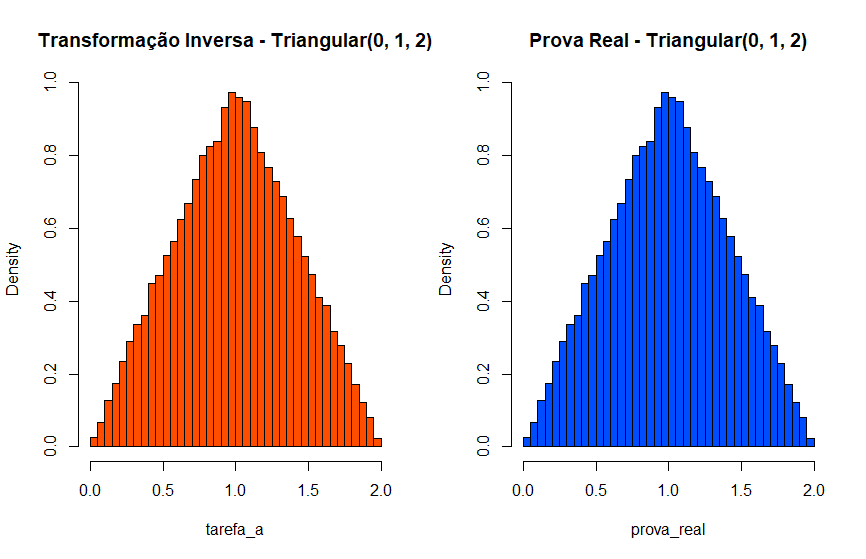
\includegraphics[width=1\linewidth]         {image.png}

\newpage
\subsection*{b) Compare com os resultados de \textit{extraDistr::rtriang} do R [...]. Dica: use o teste de KS (Kolmogorov–Smirnov).}
\textbf{Resposta:}
Retorno do teste de KS:
\[ \delta = 0.00406 \]
$ \delta $ representa a maior diferença absoluta entre funções. Sendo um valor muito próximo de zero, o teste indica que as distribuições são muito semelhantes.

\[ \pi = 0.8044, \alpha = 0.05 \]
\[ H0: x = y \]   
\[ H1: x \neq y \]  
(H0 propõe que as duas amostras provêm da mesma distribuição, enquanto H1 propõe que as duas amostras não provêm da mesma distribuição)
\[ \pi > \alpha \]
Ou seja: Não existem evidências para rejeitar H0. O resultado do teste de KS indica que provavelmente as duas amostras provêm da mesma distribuição.
\newpage
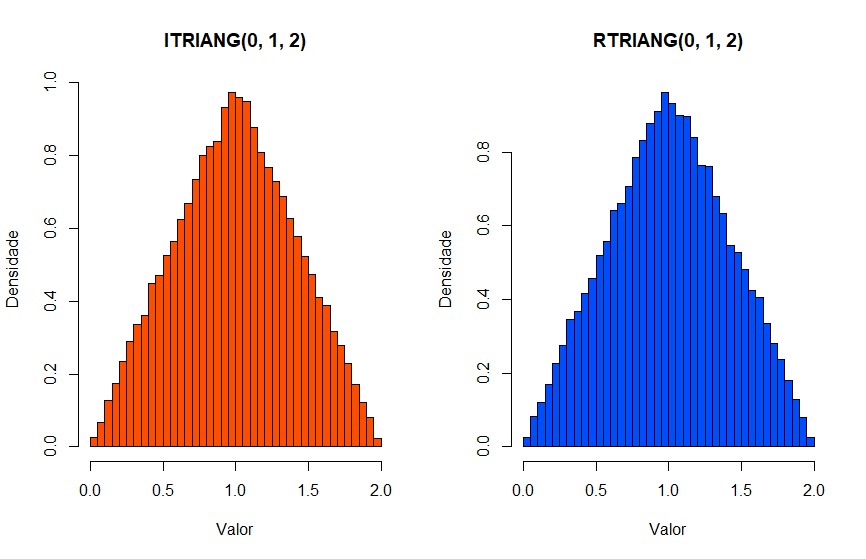
\includegraphics[width=1\linewidth]{image2.png}

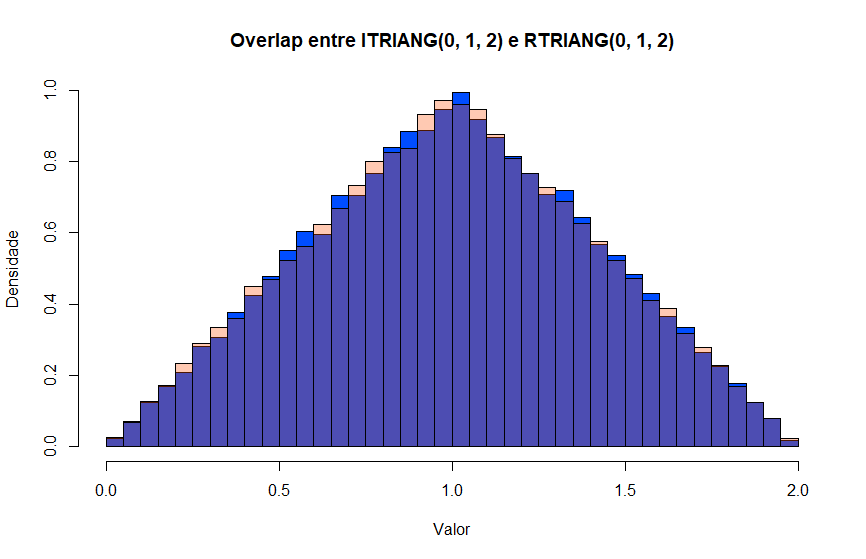
\includegraphics[width=1\linewidth]{image3.png}

\newpage

\section*{Questão 2 - Considere a tabela de dígitos aleatórios em anexo no documento de apresentação do trabalho.}
\subsection*{a) Defina uma regra para ler a tabela com o intuito de gerar valores em uma $\mathcal{U}$(0, 1).}

\textbf{Resposta:}
Ler por coluna os primeiros e os últimos elementos verticais dos grupos.

\includegraphics[width=1\linewidth]{Tabela de digitos aleatórios.png}

\subsection*{b) Liste os 5 primeiros valores obtidos a partir da regra definida no item anterior.}
\textbf{Resposta:}


\[
b = \begin{bmatrix}
57 & 80 & 22 & 18 & 53
\end{bmatrix}
\]
\subsection*{c) Utilizando o resultado do item anterior, gere 5 valores aleatórios de X tal que 
\[
X | \theta = 0.3 \sim \text{Bernoulli}(0.3)
\]}

\textbf{Resposta:}

\[
b = \begin{bmatrix}
57 & 80 & 22 & 18 & 53
\end{bmatrix}
\]

\[
\begin{array}{ll}
00 \leq b \leq 29 & x = 1 \\
30 \leq b \leq 99 & x = 0 \\
\end{array}
\]

Logo:
\[
x = \begin{bmatrix}
0 & 0 & 1 & 1 & 0
\end{bmatrix}
\]

\subsection*{d) Repita o item anterior, mas agora gerando 5 valores aleatórios de X tal que
\[
X| \theta = 0.3, n = 2 \sim \text{Binomial}(2, 0.3)
\]}

\textbf{Resposta:}


\[
b = \begin{bmatrix}
57 & 80 & 22 & 18 & 53
\end{bmatrix}
\]
\[
c = \begin{bmatrix}
40 & 54 & 89 & 00 & 97
\end{bmatrix}
\]
Admitindo como como regra:
\[
\begin{array}{ll}
00 \leq b \leq 29 & x_1 = 1 \\
30 \leq c \leq 99 & x_2 = 0 \\        
00 \leq b \leq 29 & x_1 = 1 \\
30 \leq c \leq 99 & x_2 = 0 \\
\end{array}
\]
resulta:
\[
x_1 = \begin{bmatrix}
0 & 0 & 1 & 1 & 0
\end{bmatrix}
\]
\[
x_2 = \begin{bmatrix}
0 & 0 & 0 & 1 & 0
\end{bmatrix}
\]
Somando as duas listas:

\[
x = \begin{bmatrix}
0 & 0 & 1 & 2 & 0
\end{bmatrix}
\]

\section*{Questão 3 - Explique com suas palavras.}
\subsection*{a) O que é Inferência Comparada.}
\textbf{Resposta:}

Inferencia comparada é o estudo comparativo abordagens estatísticas diferentes, como estatística bayesiana e estatística clássica, permitindo que, após esses estudos, o aluno tenha conhecimento entre pontos fortes e fracos das escolas, para que assim, suas decisões durante uma análise estatística tenham embasamento crítico, permitindo que o aluno desenvolva soluções híbridas com embasamento teórico sólido.

\subsection*{b)  Indique os principais pontos de discordância entre as inferências Clássica e Bayesiana}
\textbf{Resposta:}

A estatística bayesiana aceita e formaliza a subjetividade no seu modelo estatístico. A estatística clássica não formaliza subjetividade no seu modelo, no entanto, a subjetividade na escola clássica ainda é presente no processo analítico, como nos procedimentos de amostragem.

\subsection*{c) Explique por que precisamos dos Métodos de Monte Carlo.}
\textbf{Resposta:}

Os métodos de Monte Carlo nos permite simular áreas de integrais definidas complexas a partir de uma amostragem aleatória, sendo assim, o método de Monte Carlo nos permite evitar calcular a integral de normalização de uma posteriori.

\subsection*{d) Apresente os dois passos básicos do método de Monte Carlo. Exemplifique considerando os passos do Método da Transformação Inversa.}
\textbf{Resposta:}

\begin{enumerate}
\item Obter uma variável pseudo-aleatória uniformemente distribuída entre 0 e 1;
\item Parametrizar uma função determinística com a variável coletada.
\end{enumerate}

Para exemplificar utilizando o Método da Transformação Inversa, a Inversa da Função de Distribuição Acumulada será considerada como a função determinística do segundo passo.

\[F(x) = 1 - e^{\lambda x}\]
\[F^{-1}(u) = \frac{1}{\lambda} \text{ln}(1-u)\]

Aplicando um valor pseudo-aleatório uniformemente distribuído entre 0 e 1, é possível gerar um valor aleatório pertencente à distribuição sendo estudada. Repetindo esses passos $n$ vezes, é possível simular e aproximar a área da distribuição. 

\newpage
\begin{lstlisting}[language=R, caption={Questão 1 a) e b)}]
# Imports
library(EnvStats)
library(extraDistr)
library(stats)

# Parametros 
a <- 0
b <- 2
m <- 1
n <- 5000
set.seed(222)
u <- runif(n)

# Funcao para inversao da distribuicao triangular. Calcula F^-1(u)

itriang <- function(u, a = -1, b = 1, m = (a + b)/2)
{
  fdc <- (m - a) / (b - a)
  ifelse(u < fdc,
         a + sqrt(u * (m - a) * (b - a)),
         b - sqrt((1 - u) * (b - m) * (b - a)))
}

#******************************************************************************************************
# a) Simule a densidade de uma Triangular(0, 1, 2) a partir do Metodo da Transformacao Inversa
#******************************************************************************************************

## Execucao exercicio
tarefa_a <- itriang(u, a, b, m)

## Plotando grafico
hist(x,
     40,
     freq = FALSE,
     col = rgb(1, 0.3, 0),
     xlim = c(a, b),
     main = 'Transformacao Inversa - Triangular(0, 1, 2)'
     )

## "Prova real"
prova_real <- qtri(p=u, min=a, max=b, mode=m)

par(mfrow = c(1, 2))
hist(tarefa_a,
     40,
     freq = FALSE,
     col = rgb(1, 0.3, 0),
     xlim = c(a, b),
     main = 'Transformacao Inversa - Triangular(0, 1, 2)'
     )

hist(prova_real,
     40,
     freq = FALSE,
     col = rgb(0, 0.3, 1),
     xlim = c(a, b),
     main = 'Prova Real - Triangular(0, 1, 2)'
     )
par(mfrow = c(1, 1))

#******************************************************************************************************
# b) Compare com os resultados de extraDistr::rtriang do R [...]. Dica: use o teste de KS
#******************************************************************************************************
## Execucao exercicio
x <- itriang(u, a, b, m)
y <- rtriang(n, a, b, m)

## Plotando grafico
par(mfrow = c(1, 2))
hist(x, 40,
     freq = FALSE,
     col = rgb(1, 0.3, 0), 
     xlim = c(a, b),
     main = 'ITRIANG(0, 1, 2)',
     xlab = 'Valor',
     ylab = 'Densidade'
     )

hist(y, 40,
     freq = FALSE,
     col = rgb(0, 0.3, 1),
     xlim = c(a, b),
     main = 'RTRIANG(0, 1, 2)',
     xlab = 'Valor', ylab = 'Densidade'
)
par(mfrow = c(1, 1))

# Overlap (para identificar D)
hist(y, 40,
     freq = FALSE,
     col = rgb(0, 0.3, 1),
     xlim = c(a, b),
     main = 'Overlap entre ITRIANG(0, 1, 2) e RTRIANG(0, 1, 2)',
     xlab = 'Valor', ylab = 'Densidade'
)

hist(x, 40,
     freq = FALSE,
     col = rgb(1, 0.3, 0, 0.3), 
     xlim = c(a, b),
     xlab = 'Valor',
     ylab = 'Densidade',
     add = TRUE
)

## Teste KS
ks.test(x, y)
\end{lstlisting}
\end{document}
